%%%%%%%%%%%%%%%%%%%%%%%%%%%%%%%%%%%%%%%%%%%%%%%%%%%%%%%%%%%%%%%%%%%%%%%%%%%%%%%%
%                                                                              %
% Copyright (C) 2011-2014 Cassio Neri Moreira                                  %
%                                                                              %
% This work is licensed under a Creative Commons Attribution-ShareAlike 4.0    %
% International License.                                                       %
% http://creativecommons.org/licenses/by-sa/4.0/                               %
%                                                                              %
% The most updated version can be found at                                     %
% http://github.com/cassioneri/Efron                                           %
%                                                                              %
%%%%%%%%%%%%%%%%%%%%%%%%%%%%%%%%%%%%%%%%%%%%%%%%%%%%%%%%%%%%%%%%%%%%%%%%%%%%%%%%

\documentclass[a4paper]{article}

\usepackage[colorlinks=true,dvips]{hyperref}
\usepackage{graphicx}
\usepackage{amsmath,amsfonts,amssymb}
\usepackage{float}

\setlength{\hoffset}{0pt}
\setlength{\voffset}{0pt}
\setlength{\marginparsep}{0pt}
\setlength{\marginparwidth}{0pt}
\setlength{\evensidemargin}{0pt}
\setlength{\oddsidemargin}{0pt}
\setlength{\topmargin}{0pt}
\setlength{\textwidth}{\paperwidth}
\addtolength{\textwidth}{-2in}
\setlength{\textheight}{\paperheight}
\addtolength{\textheight}{-2in}
\addtolength{\textheight}{-\footskip}
\addtolength{\textheight}{-\headheight}
\addtolength{\textheight}{-\headsep}

\parskip.5\baselineskip

\renewcommand{\familydefault}{\sfdefault}

\title{On Continuous Efron's Dice\footnote{%
  This work is licensed under a \href{http://creativecommons.org/licenses/by-sa/4.0/}{Creative Commons Attribution-ShareAlike 4.0 International License}%
}}
\author{Cassio Neri}
\date{20 November 2011}

\hypersetup{  
  pdfinfo={  
    Title={On Continuous Efron's dice},  
    Author={Cassio Neri},
    Subject={Probability},
    Keywords={Efron's dice, Non-transitive random variables}
  }  
} 

\begin{document}

\maketitle

\begin{abstract}
A die $D_1$ is said to be {\bf stronger} than another die $D_2$ if the propability of $D_1$ beating $D_2$ is bigger than $1/2$.
It is natural to expect that being stronger is a transitive relationship, that is, if $D_1$ is stronger than $D_2$ and $D_2$ is stronger than $D_3$, then $D_1$ is stronger than $D_3$.
Efron's dice are a set of four dice invented by Bradley Efron which is a counter-example for the transitivity \cite{Wikipedia}.

In this document, instead of a set of four dice, we consider a set of independent continuous random variables $X_1$, ..., $X_M$ such that $P(X_1 > X_2) = \dots = P(X_{M - 1} > X_M) = P(X_M > X_1) = p$.
Under certain technical assumptions, we shall see that $p\le 3/4$.
\end{abstract}



\section{Introduction}

A more serious title for this document could be ``On non-transitive continuous random variables''.
However, I think that invoking the Efron's dice in the title is more appealing since this is a (literally) more concrete example of non-transitive random variables.

This document does not pretend to be a research paper.
It considers the problem with a certain degree of mathematical rigorousness and generality and, at the same time, keeping things simple.
Whenever generality is at the expense of clarity, the latter is favoured.
A few remarks along the text indicate possible gerenalisations.

We are interested in a set of independent random variables $X_1$, ..., $X_M$ such that $P(X_1 > X_2) = \dots = P(X_{M - 1} > X_M) = P(X_M > X_1) = p$.
We shall call {\bf non-transitive} to any set of random variables that satisfies this property.
The probability $p$ will be the called the {\bf winning} probability.

In the original Efron's dice problem, we have $M = 4$ and the random variables are the outcomes of four non-standard and specially built dice for which $p = 2/3$.
The peculiarity of such dice is not that they are ``unfair'' and favour some faces in respect to others.
All faces are equally probable but the numbers printed on them are not mutually distinct in $\{1, 2, 3, 4, 5, 6\}$.
This is what makes some outcomes more likely than others.
In other words, the probability space of each die is the set of six uniformly distributed faces which we can still number $1$, ..., $6$ but the random variables are not as those of a normal die where the $i^\text{th}$ face is mapped to the number $i$.
This fact will have a continuous counterparty as we shall see in Section \ref{sec:generic_case}.

Can the dice be built in order to get $p > 2/3$?
A negative answer was given by Samson \cite{Samson2011}.
He also considered the generalization for $M$ dice each of them having $N$ equally probable faces.
He showed that in the this case we have
\[
p < \frac34 - \frac1{2N} - \frac1{4N^2},
\]
and noted that $p\rightarrow 3/4$ as the number of sides $N$ goes to infinity.
Actually, we shall see that the upper bound $3/4$ holds for every non-trasitive set of random variables provided some mild conditions on their probability distribution functions hold.
Samson's work show that we can get as close as we want to the bound $3/4$ but I don't know whether
this bound can be reached.



\section{Visualising the dice}

In this section we shall revisit some of the ideas in Samson's proof \cite{Samson2011} using a more ``visual'' approach.
This will provide new insights that will be helpful in the continuous case.

For $m\in\{1,\dots, 4\}$, let $D^m$ denote the $m^\text{th}$ Efron's die and $d^m_i$ ($i\in\{1,\dots,6\}$) be the number on its $i^\text{th}$ face.
We assume that the numbers on each die are in non-decreasing order, that is, $d^m_i\le d^m_{i+1}$ for $m\in\{1, \dots, 4\}$ and $i\in\{1, \dots, 6\}$.

For each pair $(m,n)$, with $n \equiv m+1$ mod $4$, we consider a $6\times 6$ grid where each row (from bottom to top) represents a face of $D^m$ and each column (from left to right) represents a face of $D^n$.
The square in row $i$ and column $j$ should be painted in black if $d^m_i > d^n_j$ and in white otherwise.
The proportion of the black area with respect to $36$ -- the total area of the grid -- is the probability of $D^m$ beating $D^n$. (The remaining white area represents the probability of a tie or a loss for $D^m$.)
Some squares we will be painted in grey when, in the current analysis, we do not know or are not interested in its true colour.

For instance, the left of Figure \ref{fig:grid} shows the grid corresponding to two standard dice where $d^m_i = d^n_i = i$ for all $i\in\{1, \dots, 6\}$.
There are $15$ black squares in the grid, which means that the probability of the first die beating the second one is $15/36 = 5/12$.

The grid on the right shows the configuration corresponding to Efron's dice $C$ and $D$ as presented in \cite{Wikipedia}.
There are $24$ black squares, meaning that $C$ beats $D$ with probability $24/36=2/3$ as expected.

\begin{figure}[ht]
\hfill\includegraphics[width=6cm]{grid6.eps}
\hfill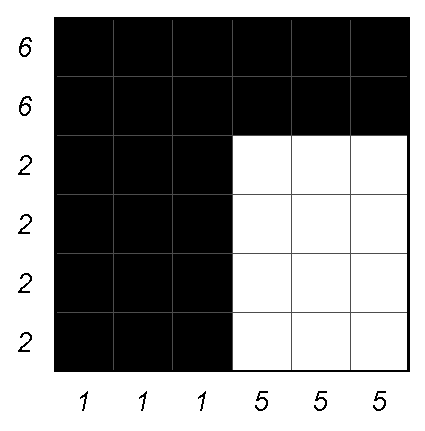
\includegraphics[width=6cm]{grid6CxD.eps}
\hfill\
\caption{Visualizing and comparing two dice.}
\label{fig:grid}
\end{figure}

Notice that, since the numbers are labeled in non-decreasing order, when a square is black, then all the squares above it or on its left must also be black.
Analogously, if a square is white, then so are all others below it or on its right.
It follows from this observation, that if the square in $3^\text{rd}$ row and $3^\text{rd}$ column is white, then at least $12$ out of the $36$ will be white as shown in Figure \ref{fig:12whites}.
Hence, at most $24$ will be black and then, the probability of $D^m$ beating $D^n$ is at most $24/36=2/3$.

\begin{figure}[ht]
\hfill\includegraphics[width=6cm]{grid6i3j3.eps}
\hfill\
\caption{If the square in $3^\text{rd}$ row and $3^\text{rd}$ column is white, then $11$ others will be so.}
\label{fig:12whites}
\end{figure}

Therefore, to make the probability of $D^m$ beating $D^n$ bigger than $2/3$ we need the square in $3^\text{rd}$ row and $3^\text{rd}$ column to be black, that is, $d^m_3 > d^n_3$.
This last inequality must hold for all $(m,n)$, with $n \equiv m+1$ mod $4$.
In other words,
\begin{equation}
\label{eq:inequalities}
d^1_3 > d^2_3 > d^3_3 > d^4_3 > d^1_3,
\end{equation}
which yields a contradiction.
We conclude that $p = 2/3$ is the sharp upper bound for the original Efron's dice problem.

Here comes the first remark regarding generalisations.
In the proof, there's nothing special about the number of dice.
Its only contribution is determining how long the sequence of inequalities 
\eqref{eq:inequalities} is.
The contradiction remains the same in any case.

Taking a step back, let's try to understand what is special about the square in $3^\text{rd}$ row and $3^\text{rd}$ column.

First of all, in order to the proof to work, the special square under consideration must be in the $i^\text{th}$ row and $j^\text{th}$ column with $i = j$.
Indeed, assuming $i\ne j$ and also that this square is black, following the previous argument, would make us conclude that $d^m_i > d^n_j$ with $i\ne j$.
This inequality would not allow us to deduce the cyclical sequence of inequalities \eqref{eq:inequalities} where all terms have the same subscript.
Hence we would not be able to deduce the absurd statement $d^m_i > d^m_i$.

Now, still following the proof, when the special square is white we conclude that there is at least a certain number of white squares.
As a consequence, we get an upper bound for the number of black squares.
To get the smallest upper bound, we need to choose the special square that  maximises the white area.

Therefore, the proof needs the special square to be the one on the left-bottom to right-top diagonal of the grid that maximizes the rectangular white area spanned by this square.
The closer the square is to the grid's centre, the bigger is this area.
Hence, the square in the $3^\text{rd}$ row and $3^\text{rd}$ column satisfies our needs.
The one on the $4^\text{th}$ row and $4^\text{th}$ column is equally adequate.

In preparation for the continuous case and overlooking the physical constraints on building dice, let's consider what happens if we increase the number of sides by splitting each of the $3^\text{rd}$ and $4^\text{th}$ faces (the {\em special ones}) into equally probable new faces.
The new grid representation for such situation is shown on the left of Figure \ref{fig:grid8}.

\begin{figure}[ht]
\hfill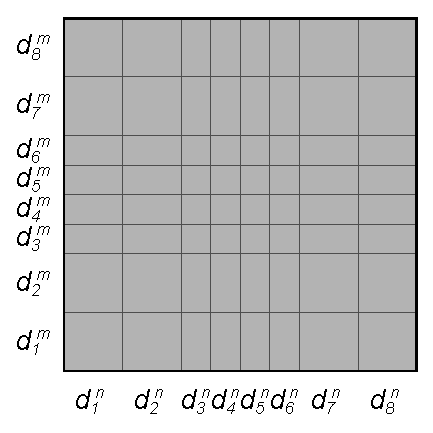
\includegraphics[width=6cm]{grid8.eps}
\hfill\includegraphics[width=6cm]{grid8i4j4.eps}
\hfill\
\caption{Fictitious dice with 8 faces.}
\label{fig:grid8}
\end{figure}

From the analysis of the proof we can immediately spot the the new special squares are the $4^\text{th}$ and $5^\text{th}$ on the left-bottom to right-top diagonal.
Picking up the $4^\text{th}$ one and assuming it's white, we obtain a white area of at least $3.5\times 3 = 10.5$.
This is illustrated on the right of Figure \ref{fig:grid8}.
The figure also emphasizes the extra grey area measuring $1.5$ that was white in Figure \ref{fig:12whites}.
Actually, this area can be black, increasing the probability $p$ by $3/2$ to $2/3 + 3/2 = 5 / 6$.

We stress that the previous arguments on the fictitious dice does not say that the upper bound for the winning probability is achieved.
The problem is not the physical impossibility of building such dice because we could use another set of random variables. (Actually, we are already doing it by considering the grid with the Lebesgue measure.)
The argument just gives just an upper bound for winning probability for a certain set of random variables.



\section{General non-transitive random variables}
\label{sec:generic_case}

In this section we adapt the previous ideas to non-transitive random variables that are not necessarily discrete as in the dice case.
We make two assumptions on the set of non-transitive random variables $X_1$, ..., $X_M$, namely,
\begin{enumerate}
\item\label{it:space} They are defined on the probability space $]0, 1[^M$ equipped with the Lebesgue $\sigma$-algebra and (probability) measure.
\item\label{it:form} For all $(x_1, ..., x_M)\in\ ]0, 1[^M$, $X_m(x_1, ..., x_M) = F_m(x_m)$, where $F_m:]0, 1[\rightarrow\mathbb{R}$ is non-decreasing.
\end{enumerate}

These assumptions say that each $X_m$ is a function of an uniformly distributed random variable $x_m$ in $]0, 1[$.
Notice the similarity with the original Efron's dice where the random variables are functions of uniformly random distributed faces of a die.

We shall prove that $3/4$ is an upper bound for the winning probability.

For each pair $(m, n)$, with $n \equiv m + 1$ mod $M$, the grid used in the previous argument becomes the square $]0, 1[\times]0, 1[$ where each point $(x_m, x_n)$ is painted in black if $F_m(x_m) > F_n(x_n)$ and in white otherwise.
In more mathematical terms, we consider the set $B_{m,n} = \{(x_m, x_n)\in\ ]0, 1[\times ]0, 1[\ ;\ F_m(x_m) > F_n(x_n)\}$ whose Lebesgue measure is the winning probability $p = P(X_m > X_n)$ of $X_m$ beating $X_n$.

The proof here also needs its special ``square'' which, for the continuous case, collapses into the single point $(1/2, 1/2)$.

Suppose that there exists a pair $(m, n)$, with $n \equiv m + 1$ mod $M$, such that $F_m(1/2) \le F_n(1/2)$ (that is, $(1/2, 1/2)$ is white in this grid).
Since $F$ is non-decreasing we have
\[
F_m(x_m) \le F_m(1/2) \le F_n(1/2) \le F_n(x_n), \quad \forall x_m\in\ ]0, 1/2[, \quad \forall x_n\in\ ]1/2, 1[.
\]
It follows that
\[
A_{m, n} := \{x\in\ ]0, 1[^M\ ;\ x_m\in\ ]0, 1/2[,\ x_n\in\ ]1/2, 1[\} \subset B_{m, n}^\complement.
\]
Hence, $1/4 = P(A_{m, n})\le P(B_{m,n}^\complement) = P(X_m \le X_n)$ and then, $p = P(X_m > X_n)\le 3/4$.

We conclude that if $p > 3/4$, then $F_m(1/2) > F_n(1/2)$ for all $(m, n)$, such that $n \equiv m + 1$ mod $M$.
Therefore,
\[
F_1(1/2) > F_2(1/2) > \dots > F_M(1/2) > F_1(1/2)
\]
which is absurd.

We end this document by noticing that we can replace the hypothesis on $X_1$, ..., $X_M$ stated at the beginning of this section by a simple assumption on the their probability distribution functions.
This means that the same bound on the winning probability hold for a larger collection of continuous random variables.

Indeed, let $G_m$ be the probability distribution function of $X_m$ and {\bf assume that $G_m$ is continuous and strictly increasing.}
Then $G_m:\mathbb{R}\rightarrow]0, 1[$ is invertible with inverse $F_m := G_m^{-1}:]0, 1[\rightarrow\mathbb{R}$.

We denote by $x := (x_1, ..., x_M)$ a generic point in the probability space $]0, 1[^M$ equipped with the Lebesgue $\sigma$-algebra and (probability) measure.
Notice that the projections $\pi_m:]0, 1[^M\rightarrow]0, 1[$ given by $\pi_m(x) := x_m$, $m\in\{1, ..., M\}$, are independent and uniformly distributed in $]0, 1[$.

Hence, the variables $\tilde X_1$, ..., $\tilde X_M$ defined by $\tilde X_m(x) := F_m(x_m)$ for all $m\in\{1, ..., M\}$ satisfy the conditions \ref{it:space} and \ref{it:form} above.
Moreover $\tilde X_m$ is equal in distribution to $X_m$ since
\[
P(\tilde X_m < y) = P(F_m(x_m) < y) = P(x_m < G_m(y)) = P(\pi_m(x) < G_m(y)) = G_m(y),
\]
where the last equality is a consequence of $\pi_m$ being uniformly distributed in $]0, 1[$.

Therefore, the result $p\le 3/4$ still holds in this case.

I feel that these results can be extended further without the need for strictly monotonicity of $G_m$ but the proof must deal carefully with intervals where $G_m$ is constant because they complicate the inversion of $G_m$.



\begin{thebibliography}{99}

\bibitem{Wikipedia} Wikepedia, {\em Nontransitive dice}, \url{http://en.wikipedia.org/wiki/Nontransitive_dice#Efron.27s_dice}.

\bibitem{Samson2011} Ophir Samson, {\em Efron�s Dice}, \url{http://ophir-research.com/Papers/Efron.pdf}.

\end{thebibliography}

\end{document}
